\documentclass[runningheads,a4paper]{llncs}

\usepackage[cmex10]{amsmath}
\usepackage{graphicx}
\usepackage{booktabs}
\usepackage{tabularx}
\usepackage{color}
\usepackage{subfig}
\usepackage[unicode,
					  colorlinks,
						linkcolor={red},
						citecolor={blue},
						urlcolor={blue},
            pdfauthor={Maciej Piernik, Arkadiusz Jachnik},
            pdftitle={State--changing sequential pattern mining using uplift modeling},
            pdfsubject={Sequential pattern mining},
            pdfkeywords={sequential patterns, uplift modeling}]{hyperref}

\newcolumntype{R}{>{\raggedleft\arraybackslash}X}
\newcommand{\argmax}[1]{\underset{#1}{\operatorname{argmax}}\;}
\newcommand{\matr}[1]{\mathbf{#1}}

\begin{document}

\mainmatter

\title{State--changing sequential pattern mining using uplift modeling}

\titlerunning{State--changing sequential patterns}

\author{Maciej Piernik \and Arkadiusz Jachnik}

\authorrunning{Maciej Piernik \and Arkadiusz Jachnik}

\institute{Institute of Computing Science, Poznan University of Technology\\
ul. Piotrowo 2, 60--965 Poznan, Poland\\
\email{maciej.piernik@cs.put.poznan.pl}}

\maketitle

\begin{abstract}

\keywords{sequential patterns, uplift modeling}
\end{abstract}

\section{Introduction}
\label{sec:introduction}
%More and more data generated every day come in the form of sequences.
%Examples...
%With such prevalence, many types of analyses are possible, including classification, clustering, and outlier detection.
%However, probably the most studied field of sequential data processing is sequential pattern mining.

Sequential patterns are an extension of frequent patterns (or frequent itemsets, known from association rule mining) to sequential data.
They find many applications in domains such as customer transaction analysis, web mining, software bug analysis, chemical and biological analysis~\cite{Aggarwal:2014}.
Just like with traditional frequent patterns, there are many versions of sequential patterns, depending on the structure of the sequences.
For instance, each event in a sequence can be either a single item or an itemset; the precedence of elements can be implied solely by their order or explicitly by time; time can be used to further narrow the problem by constraining time gaps between elements; each event in a sequence can be described by a symbol, a number, or a set of features, etc.~\cite{Dong:2009}.
On top of that, in scenarios such as classification, class information can be added to each element in each sequence.
This results in a setting where a dataset contains sequences of pairs $\langle\texttt{event}, \texttt{class}\rangle$.
In many real-world scenarios, however, such a setting is impossible to achieve, as the class information may be provided with a delay or even completely asynchronously from the analyzed events.
Consider a sequence of treatments prescribed to a given patient for a certain disease measured by some indicator (e.g., blood pressure).
After a series of events (e.g., pharmaceuticals, medical procedures, dietary regulations) the indicator may either improve, worsen, or stay unchanged.
However, this result does not necessarily coincide with any of the events nor need it be a result of one, all, or any of the events.
This scenario is universal when modeling people's behavior, opinion, or --- more generally speaking --- \textit{state}.
As illustrated by the examples above, this problem is no longer described by a single sequence of events (like in classical sequential pattern mining), but rather by two connected sequences --- one with the events and the other with classes.
To the best of our knowledge, processing of sequential data of such composition has not yet been considered and is the focus of this research.

The assumption underlying the described scenario is that the events in the sequences influence the outcomes registered by the classes.
A classical example of such an analysis performed on traditional data is the aforementioned clinical trial.
In order to properly model the outcomes of patients' treatments, the results need to be evaluated against a control group.
A method aiming specifically at this task is uplift modeling, as it's goal, as originally formulated, is to model the \textit{change} in peoples' behavior as a result of intentional activity~\cite{Radcliffe:1999}.

In this paper, we propose a solution to the problem of state--changing sequential pattern mining.
Our method is designed to work in a setting where the information about states (classes) is provided separately from the underlying sequence of events.
Inspired by clinical trials, it relies on the notion of control group and uses uplift modeling to factor this notion into the processing.
We experimentally evaluate our proposal using real-world data to showcase its superiority w.r.t. traditional sequential patterns in the described scenarios.

The remainder of this paper is organized as follows.
Section~\ref{sec:related} outlines the research related to our proposal.
In Section~\ref{sec:main}, we formally define state--changing sequential patterns and show how to find them.
In Section~\ref{sec:experiments}, we experimentally evaluate our proposal and discuss the obtained results.
Finally, in Section~\ref{sec:conclusions}, we conclude the paper and draw lines of future research.

\section{Related Work}
\label{sec:related}

\section{Sequential pattern mining with uplift measure}
\label{sec:main}

\begin{figure}[!ht]
	\centering
		%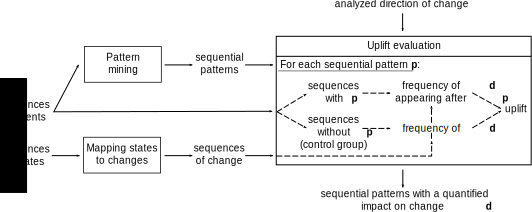
\includegraphics[width=0.9\textwidth]{images/concept}
	\caption{Illustration of the proposed method}
	\label{fig:concept}
\end{figure}
\vspace{-10pt}

\section{Experiments}
\label{sec:experiments}
\subsection{Experimental Setup}

Fig.~\ref{fig:setup} depicts the experimental procedure.
\begin{figure}[h]
	\centering
		%\includegraphics[width=0.60\textwidth]{images/setup}
	\caption{Experimental procedure}
	\label{fig:setup}
\end{figure}

\subsection{Datasets}

\begin{table}[htbp]
	\scriptsize
  \centering
  \caption{Characteristics of datasets}
    \begin{tabularx}{\textwidth}{l@{}R@{}R@{}R@{}}
		\toprule
    Dataset  & \#Instances & Avg. seq. len. & \#Classes \\
		\midrule

    \bottomrule
    \end{tabularx}%
  \label{tab:datasets}%
\end{table}%

\subsection{Results}

\section{Conclusions}
\label{sec:conclusions}


\subsubsection*{Acknowledgments.} This research is partly funded by the Polish National Science Center under Grant No. DEC-2015/19/B/ST6/02637.

\bibliographystyle{splncs}
\bibliography{Bibliography}

\end{document}
